% LaTeX source for ``Modeling and Simulation in Python''
% Copyright 2017  Allen B. Downey.

% License: Creative Commons Attribution-NonCommercial 3.0 Unported License.
% http://creativecommons.org/licenses/by-nc/4.0/
%

\documentclass[12pt]{book}

\title{Modeling and Simulation in Python}
\author{Allen B. Downey}

\newcommand{\thetitle}{Modeling and Simulation in Python}
\newcommand{\thesubtitle}{}
\newcommand{\theauthors}{Allen B. Downey}
\newcommand{\theversion}{0.0.1}


%%%% Both LATEX and PLASTEX

\usepackage{graphicx}
\usepackage{hevea}
\usepackage{makeidx}
\usepackage{setspace}
\usepackage{xcolor}
\usepackage{upquote}
\usepackage[listings]{tcolorbox}
\usepackage{siunitx}

\definecolor{light-gray}{gray}{0.95}

\newtcblisting{python}{
  skin=standard,
  boxrule=0.4pt,
  colback=light-gray,
  listing only,
  top=0pt,
  bottom=0pt,
  left=0pt,
  right=0pt,
  boxsep=2pt,
  listing options={
    basicstyle=\ttfamily,
    language=python,
    showstringspaces=false,
  },
}
 
\newtcblisting{result}{
  skin=standard,
  boxrule=0.0pt,
  colback=white,
  listing only,
  top=0pt,
  bottom=0pt,
  left=0pt,
  right=0pt,
  boxsep=2pt,
  listing options={
    basicstyle=\ttfamily,
    language=python,
    showstringspaces=false,
  },
}
 
\makeindex

% automatically index glossary terms
\newcommand{\term}[1]{%
\item[#1:]\index{#1}}

\usepackage{amsmath}
\usepackage{amsthm}

% format end of chapter excercises
\newtheoremstyle{exercise}
  {12pt}        % space above
  {12pt}        % space below
  {}            % body font
  {}            % indent amount
  {\bfseries}   % head font
  {}            % punctuation
  {12pt}        % head space
  {}            % custom head
\theoremstyle{exercise}
\newtheorem{exercise}{Exercise}[chapter]

\newif\ifplastex
\plastexfalse

%%%% PLASTEX ONLY
\ifplastex

\usepackage{localdef}

\usepackage{url}

\newcount\anchorcnt
\newcommand*{\Anchor}[1]{%
  \@bsphack%
    \Hy@GlobalStepCount\anchorcnt%
    \edef\@currentHref{anchor.\the\anchorcnt}%
    \Hy@raisedlink{\hyper@anchorstart{\@currentHref}\hyper@anchorend}%
    \M@gettitle{}\label{#1}%
    \@esphack%
}

% code listing environments:
% we don't need these for plastex because they get replaced
% by preprocess.py
%\newenvironment{code}{\begin{code}}{\end{code}}
%\newenvironment{stdout}{\begin{code}}{\end{code}}

% inline syntax formatting
\newcommand{\py}{\verb}%}

%%%% LATEX ONLY
\else

\input{latexonly}

\fi

%%%% END OF PREAMBLE
\begin{document}

\frontmatter

%%%% PLASTEX ONLY
\ifplastex

\maketitle

%%%% LATEX ONLY
\else

\begin{latexonly}

%-half title--------------------------------------------------
\thispagestyle{empty}

\begin{flushright}
\vspace*{2.0in}

\begin{spacing}{3}
{\huge \thetitle}
\end{spacing}

\vspace{0.25in}

Version \theversion

\vfill

\end{flushright}

%--verso------------------------------------------------------

\newpage
\newpage
%\clearemptydoublepage
%\pagebreak
%\thispagestyle{empty}
%\vspace*{6in}

%--title page--------------------------------------------------
\pagebreak
\thispagestyle{empty}

\begin{flushright}
\vspace*{2.0in}

\begin{spacing}{3}
{\huge \thetitle}
\end{spacing}

\vspace{0.25in}

Version \theversion

\vspace{1in}


{\Large
\theauthors \\
}


\vspace{0.5in}

{\Large Green Tea Press}

{\small Needham, Massachusetts}

%\includegraphics[width=1in]{figs/logo1.eps}
\vfill

\end{flushright}


%--copyright--------------------------------------------------
\pagebreak
\thispagestyle{empty}

Copyright \copyright ~2016 \theauthors.



\vspace{0.2in}

\begin{flushleft}
Green Tea Press       \\
9 Washburn Ave \\
Needham MA 02492
\end{flushleft}

Permission is granted to copy, distribute, transmit and adapt this work under a Creative Commons Attribution-NonCommercial-ShareAlike 4.0 International License: \url{http://creativecommons.org/licenses/by-nc-sa/4.0/}.

If you are interested in distributing a commercial version of this
work, please contact the author.

The \LaTeX\ source for this book is available from

\begin{code}
      http://greenteapress.com/complexity
\end{code}

%--table of contents------------------------------------------

\cleardoublepage
\setcounter{tocdepth}{1}
\tableofcontents

\end{latexonly}


% HTML title page------------------------------------------

\begin{htmlonly}

\vspace{1em}

{\Large \thetitle}

{\large \theauthors}

Version \theversion

\vspace{1em}

Copyright \copyright ~2017 \theauthors.

Permission is granted to copy, distribute, and/or modify this work
under the terms of the Creative Commons
Attribution-NonCommercial-ShareAlike 4.0 International License, which is
available at \url{http://creativecommons.org/licenses/by-nc-sa/4.0/}.

\vspace{1em}

\setcounter{chapter}{-1}

\end{htmlonly}

% END OF THE PART WE SKIP FOR PLASTEX
\fi

\chapter{Preface}
\label{preface}

Usual rant about freshman physics.

\section{Who is this book for?}

No Python.

High school physics and high school calc, but not really.


\section{Using the code}
\label{code}

The code and sound samples used in this book are available from
\url{https://github.com/AllenDowney/ModSimPy}.  Git is a version
control system that allows you to keep track of the files that
make up a project.  A collection of files under Git's control is
called a ``repository''.  GitHub is a hosting service that provides
storage for Git repositories and a convenient web interface.
\index{repository}
\index{Git}
\index{GitHub}

The GitHub homepage for my repository provides several ways to
work with the code:

\begin{itemize}

\item You can create a copy of my repository
on GitHub by pressing the {\sf Fork} button.  If you don't already
have a GitHub account, you'll need to create one.  After forking, you'll
have your own repository on GitHub that you can use to keep track
of code you write while working on this book.  Then you can
clone the repo, which means that you copy the files
to your computer.
\index{fork}

\item Or you could clone
my repository.  You don't need a GitHub account to do this, but you
won't be able to write your changes back to GitHub.
\index{clone}

\item If you don't want to use Git at all, you can download the files
in a Zip file using the button in the lower-right corner of the
GitHub page.

\end{itemize}

All of the code is written to work in both Python 2 and Python 3
with no translation.

I developed this book using Anaconda from
Continuum Analytics, which is a free Python distribution that includes
all the packages you'll need to run the code (and lots more).
I found Anaconda easy to install.  By default it does a user-level
installation, not system-level, so you don't need administrative
privileges.  And it supports both Python 2 and Python 3.  You can
download Anaconda from \url{http://continuum.io/downloads}.
\index{Anaconda}

If you don't want to use Anaconda, you will need the following
packages:

\begin{itemize}

\item NumPy for basic numerical computation, \url{http://www.numpy.org/};
\index{NumPy}

\item SciPy for scientific computation,
  \url{http://www.scipy.org/};
\index{SciPy}

\item matplotlib for visualization, \url{http://matplotlib.org/}.
\index{matplotlib}

%TODO: what else

\end{itemize}

Although these are commonly used packages, they are not included with
all Python installations, and they can be hard to install in some
environments.  If you have trouble installing them, I
recommend using Anaconda or one of the other Python distributions
that include these packages.
\index{installation}

The code for each chapter, and starter code for the exercises, is in
Jupyter notebooks.  If you have not used Jupyter before, you can read
about it at \url{http://jupyter.org}.  \index{Jupyter}

There are three ways you can work with the Jupyter notebooks:

\begin{description}

\item[Run Jupyter on your computer]

If you installed Anaconda, you
  probably got Jupyter by default.  To check, start the server from
the command line, like this:

\begin{verbatim}
$ jupyter notebook
\end{verbatim}

If it's not installed, you can install it in Anaconda like this

\begin{verbatim}
$ conda install jupyter
\end{verbatim}

When you start the server, it should launch your default web browser
or create a new tab in an open browser window.

\item[Run Jupyter on Binder]

Binder is a service that runs Jupyter in a virtual machine.  If you
follow this link, \url{http://mybinder.org/repo/AllenDowney/ModSimPy},
you should get a Jupyter home page with the notebooks for this book
and the supporting data and scripts.

You can run the scripts and modify them to run your own code, but the
virtual machine you run in is temporary.  Any changes you make will
disappear, along with the virtual machine, if you leave it idle for
more than about an hour.

\item[View notebooks on nbviewer]

When we refer to notebooks later in the book, we will provide links to
nbviewer, which provides a static view of the code and results.  You
can use these links to read the notebooks and listen to the examples,
but you won't be able to modify or run the code, or use the
interactive widgets.

\end{description}

Good luck, and have fun!



\section*{Contributor List}

If you have a suggestion or correction, send it to 
{\tt downey@allendowney.com}.  If I make a change based on your
feedback, I will add you to the contributor list
(unless you ask to be omitted).
\index{contributors}

If you include at least part of the sentence the
error appears in, that makes it easy for me to search.  Page and
section numbers are fine, too, but not as easy to work with.
Thanks!

\small

\begin{itemize}

\item My early work on this book benefited from conversations with
my amazing colleagues at Olin College, including John Geddes, Alison
Wood, Chris Lee, and Jason Woodard.

% ENDCONTRIB

\end{itemize}



\normalsize

\cleardoublepage

% TABLE OF CONTENTS
\begin{latexonly}

\tableofcontents

\cleardoublepage

\end{latexonly}

% START THE BOOK
\mainmatter


\chapter{Modeling}
\label{sounds}

Intro

\section{What is a model?}

The world is a complicated place.  In order to make sense of it, we use {\bf models}, which are generally smaller and simpler than the thing we want to study.

The word ``model" means different things in different contexts, so it is hard to define, except by example.

Some models are actual objects, like a scale model of a car, which has the same shape as the car, but smaller.  Scale models are often useful for testing properties of mechanical systems, like air resistance.

This book is about {\bf mathematical models}, which are ideas, not objects.  If you studied Newton's laws of motion, what you learned is a mathematical model of how object move in space when forces are applied to them.

For example, you might have heard that a penny dropped from the top of the Empire State Building would be going so fast when it hit the pavement that it would be embedded in the concrete; or if it hit a person, it would break their skull.

One way to test this myth is by making and analyzing a model.  For example, let's assume that the effect of air resistance is small.  This will turn out to be a bad assumption, but bear with me.  If air resistance is negligible, the primary force acting on the penny is gravity, which causes the penny to accelerate at 9.8 meters per second squared (\SI{}{\meter\per\second\squared}).

If the initial velocity is 0, the velocity after $t$ seconds is $at$, and the height the penny has dropped at $t$ is

\[ h = at^2/2 \]

Using algebra, we can solve for $t$:

\[ t = \sqrt{2h/a} \]

Plugging in $a = \SI{9.8}{\meter\per\second\squared}$ and $h=\SI{381}{\meter}$, we get $t = \SI{8.8}{\second}$.  Then computing $v=at$ we get a velocity on impact of $\SI{86}{\meter\per\second}$, which is about 190 miles per hour.  That sounds like it could hurt.

Of course, these results are not exact because the model is based on simplifications.  For example, we assume that gravity is constant.  In fact, the force of gravity is different on different parts of the globe, and gets weaker as you move away from the surface.  But these differences are small, so ignoring them is probably a good decision for this scenario.

On the other hand, ignoring air resistance is not a good decision.  Once the penny gets to about \SI{20}{\meter\per\second}, the upward force of air resistance equals the force of gravity, so the penny stops accelerating.  After that, it doesn't matter how far the penny falls; it will hit the sidewalk (or your head) at about \SI{20}{\meter\per\second}, much less than \SI{86}{\meter\per\second}, as the simple model predicts.

The statistician George Box famously said ``All models are wrong, but some are useful."  He was talking about statistical models, but his wise words apply to all kinds of models.  Our first model, which ignores air resistance, is very wrong, and probably not useful.  The second model is also wrong, but much better, and probably good enough for the purpose.

The television show {\it Mythbusters} has tested the myth of the falling penny more carefully; you can view the results at \url{https://www.youtube.com/watch?v=PHxvMLoKRWg}.  Their work is based on a mathematical model, measurements to determine the force of air resistance on a penny, and a physical model of a human head.


\section{Computation}

There are (at least) two ways to work with mathematical models, {\bf analysis} and {\bf simulation}.  Analysis often involves algebra and other kinds of symbolic manipulation.  Simulation often (but not always) involves computers.

In this book we do some analysis and a lot of simulation; along the way, we will discuss the pros and cons of each.  The primary tools we use for simulation are the Python programming language and Jupyter, which is an environment for writing and running programs.

As a first example, I'll show you how I computed the results from the previous section using Python.  You can view this example, and the other code in this chapter, at \url{FILL THIS IN}.  At the end of the chapter, I'll give you instructions for downloading and running the examples. 

First I'll created a {\bf variable} to represent acceleration.

\begin{python}
a = 9.8 * meter / second**2
\end{python}

A variable is a name that corresponds to a value.  In this example, the name is \py{a} and the value is the number \py{9.8} multiplied by the units \py{meter / second**2}.  This example demonstrates the symbols Python uses to perform mathematical operations:

\begin{tabular}{l|c}
{\bf Operation} & {\bf Symbol} \\ 
\hline 
Addition & \py{+} \\ 
Subtraction & \py{-} \\ 
Multiplication & \py{*} \\ 
Division & \py{/} \\ 
Exponentiation & \py{**}  \\ 
\end{tabular} 

Next, we can compute time it takes for the penny to drop \SI{381}{\meter}, which is the height of the Empire State Building.

\begin{python}
h = 381 * meter
t = sqrt(2 * h / a)
\end{python}

These lines create two more variables: \py{h} gets the height of the building in meters; \py{t} gets the time, in seconds, for the penny to fall to the sidewalk.  \py{sqrt} is a {\bf function} that computes square roots.  Python keeps track of units, so the result, \py{t}, has the correct units, seconds.

Finally, we can compute the velocity of the penny after $t$ seconds:

\begin{python}
v = a * t
\end{python}

The result is about \SI{86}{\meter\per\second}, again with the correct units.  This example demonstrates analysis and computation using Python.  In the next section, we will see an example of simulation.


\section{Modeling a bike share system}

Imagine a bike share system for students traveling between Olin College and Wellesley College, which are about 3 miles apart in eastern Massachusetts.

This example demonstrates the features of Python we'll use to develop computational simulations of real-world systems.  Along the way, I will make decisions about how to model the system.  In the next chapter we'll review these decisions.

Suppose the system contains 12 bikes and two bike racks, one at Olin and one at Wellesley, each with the capacity to hold 12 bikes.

As students arrive, check out a bike, and ride to the other campus,
the number of bikes in each location changes.  In the simulation,
we'll need to keep track of where the bikes are.  To do that, I'll
create a {\bf state object}:

\begin{python}
from modsim import *

bikeshare = State(olin=10, wellesley=2)
\end{python}

The first line is an {\bf import statement} that tells Python
to read {\tt modsim}, which is a collection of functions, including \py{sqrt}, which we used in the previous section, \py{State}, which we are using now, and many more.

\py{State} creates a {\bf state object} which is a collection of {\bf state variables}.  In this example, the state variables are named \py{olin} and \py{wellesley} and they represent the number of bikes at
Olin and Wellesley.  The initial values of are 10 and 2, indicating that there are 10 bikes at Olin and 2 at Wellesley.  The state object created by \py{State} is assigned to a new variable
named \py{bikeshare}.

We can read the variables inside a state object using ``dot notation'', like this:

\begin{python}
bikeshare.olin
\end{python}

The result is the value 10.  Similarly, for:

\begin{python}
bikeshare.wellesley
\end{python}

The result is 2.  If you ever forget what variables a state
object has, you can use \py{print_state}, another function from
\py{modsim}:

\begin{python}
print_state(bikeshare)
\end{python}

\py{print_state} is a function, like \py{State}.  The name in
parentheses is a function {\bf argument}, which specifies which
state object we want to print.

The result looks like this:

\begin{result}
wellesley -> 2
olin -> 10
\end{result}

We can update the state of the system by assigning new values to
the variables.  For example, if a student moves a bike from Olin
to Wellesley, we can figure out the new values and assign them:

\begin{python}
bikeshare.olin = 9
bikeshare.wellesley = 3
\end{python}

Or we could use {\bf update operators} to subtract 1 from
\py{olin} and add 1 to \py{wellesley}:

\begin{python}
bikeshare.olin -= 1
bikeshare.wellesley += 1
\end{python}

The result is the same either way.


\section{Plotting}

As the state of the system changes, it is often useful to plot the
values of the variables over time.  {\tt modsim} provides functions
we can use to create figures and plot values.

\begin{python}
newfig()
plot(bikeshare.olin, 'rs-')
plot(bikeshare.wellesley, 'bo-')
\end{python}

The first function, \py{newfig}, creates a new figure.  In Jupyter, the
behavior of this function depends on a command in the
first cell:

\begin{itemize}

\item If you want the figures to appear in the notebook, use

\begin{python}
%matplotlib notebook
\end{python}

\item If you want the figures to appear in separate windows, use

\begin{python}
%matplotlib qt
\end{python}

\end{itemize}

These commands are not actually Python; they are so-called ``magic commands" that control the behavior of Jupyter.

The next two lines plot the variables of the state object.  The
\py{plot} function takes two arguments: the first is the variable to plot;
the second is a ``style string''.  In general, a {\bf string} is a sequence of letters, numbers, and punctuation that appear in quotation marks.

A style string contains information about what the plot should
look like.  The string \py{'rs-'} means we want red squares with
lines between them; \py{'bo-'} means we want blue circles with
lines.

For more information about style strings, see
\url{https://matplotlib.org/api/pyplot_api.html#matplotlib.pyplot.plot}.

The plotting functions in {\tt modsim} are based on Pyplot, which
is part of Matplotlib, which is a Python {\bf library} for generating
figures.  To learn more about how to use these function, you can read
the Matplotlib/Pyplot documentation.


\section{Functions}

When you are developing code in Jupyter, it is often efficient to
write 1--2 lines in each cell, test them to confirm they do what
you intend, and then use them to define a new function.  For
example, these lines move a bike from Olin to Wellesley:

\begin{python}
bikeshare.olin -= 1
bikeshare.wellesley += 1
\end{python}

Rather than repeat them every time a bike moves, we can define a
new function:

\begin{python}
def bike_to_wellesley():
    bikeshare.olin -= 1
    bikeshare.wellesley += 1
\end{python}

\py{def} is a {\bf keyword} that tells Python we are defining a new
function.  The name of the function is \py{bike_to_wellesley}.
The empty parentheses indicate that this function takes no
arguments.  The colon indicates the beginning of an indented
{\bf code block}.

The next two lines are the {\bf body} of the function.  They have
to be indented; by convention, the indentation is 4 spaces.

When you define a function, it has no immediate effect.  The body
of the function doesn't run until you {\bf call} the function.
Here's how to call this function:

\begin{python}
bike_to_wellesley()
\end{python}

When you call this function, it updates the variables of the
{\tt bikeshare} state object, which you can confirm by printing
or plotting the new state.

When you call a function that takes no arguments, you have to
include the empty parentheses.  If you leave them out, like this:

\begin{python}
bike_to_wellesley
\end{python}

Python looks up the name of the function and displays:

\begin{python}
<function __main__.bike_to_wellesley>
\end{python}

This result indicates that \py{bike_to_wellesley} is a function
that belongs to a namespace called \py{__main__}.  You don't
need to know what that means, but if you see something like this,
it probably means that you looked up a function but you didn't
actually run it.  So don't forget the parentheses.


\section{Parameters}

Similarly, we can define a function that moves a bike from
Wellesley to Olin:

\begin{python}
def bike_to_olin():
    bikeshare.wellesley -= 1
    bikeshare.olin += 1
\end{python}

And run it like this:

\begin{python}
bike_to_olin()
\end{python}

One benefit of defining functions is that you avoid repeating chunks
of code, which makes programs smaller.  Another benefit is that the
name you give the function documents what it does, which makes programs
more readable.

In this example, there is one other benefit that might be even
more important.  Putting these lines in a function makes the program
more reliable because it guarantees that when we decrease the number
of bikes at Olin, we increase the number of bikes at Wellesley.
That way, we can guarantee that bikes are neither created nor
destroyed!

However, now we have two functions that are nearly identical except
for a change of sign.  Repeated code makes programs harder to work with, because if we make a change, we have to make it in several places.

We can avoid that by defining a more general function that moves any number of bikes in either direction:

\begin{python}
def move_bike(n):
    bikeshare.olin -= n
    bikeshare.wellesley += n
\end{python}

The name in parentheses, \py{n}, is a {\bf parameter} of the function.
When we run the function, the argument we provide gets assigned to
the parameter.  So if we run \py{move_bike} like this:

\begin{python}
move_bike(1)
\end{python}

It assigns the value of the argument, \py{1}, to the parameter, \py{n}, and then runs the body of the function.  So the effect is the same as:

\begin{python}
n = 1
bikeshare.olin -= n
bikeshare.wellesley += n
\end{python}

Which moves a bike from Olin to Wellesley.  Similarly, if we call
\py{move_bike} like this:

\begin{python}
move_bike(-1)
\end{python}

The effect is the same as:

\begin{python}
n = -1
bikeshare.olin -= n
bikeshare.wellesley += n
\end{python}

Which moves a bike from Wellesley to Olin.  Now that we have
\py{move_bike}, we can rewrite the other two functions to use it: 

\begin{python}
def bike_to_wellesley():
    move_bike(1)
    
def bike_to_olin():
    move_bike(-1)
\end{python}

If you define the same function name more than once, the new definition
replaces the old one.


\section{Print statements}

As you write more complicated programs, it is easy to lose track of what is going on.  One of the most useful tools for debugging is the {\bf print statement}, which displays text in the Jupyter notebook.

Normally when Jupyter runs the code in a cell, it displays the value of the last line of code.  For example, if you run:

\begin{python}
bikeshare.olin
bikeshare.wellesley
\end{python}

Jupyter runs both lines of code, but it only displays the value of the second line.

If you want to display more than one value, you can use print statements:

\begin{python}
print(bikeshare.olin)
print(bikeshare.wellesley)
\end{python}

\py{print} is a function, so it takes an argument in parentheses.  It can also take a list of arguments separated by commas, like this:

\begin{python}
print(bikeshare.olin, bikeshare.wellesley)
\end{python}

In this example, the two values appear on the same line, separated by a space.

Print statements are also useful for debugging functions.  For example, if you add a print statement to \py{move_bike}, like this:

\begin{python}
def move_bike(n):
    print('Running move_bike with n =', n)
    bikeshare.olin -= n
    bikeshare.wellesley += n
\end{python}

Each time you run \py{move_bike}, it displays a message and the value of the parameter, \py{n}.



\section{If statements}

{\tt modsim} provides a function called \py{flip} that takes
as an argument a probability between 0 and 1:

\begin{python}
flip(0.7)
\end{python}

The result is either \py{True} with probability 0.7 or \py{False} with probability 0.3.  If you ran this function 100 times, you would expect to get \py{True} about 70 times and \py{False} about 30 times.  But the results are random, so they might differ from these expectations.

\py{True} and \py{False} are special values defined by Python.  Note
that they are not strings.  There is a difference between \py{True},
which is a special value, and \py{'True'}, which is a string.

\py{True} and \py{False} are called {\bf boolean} values because
they are related to Boolean algebra (\url{https://en.wikipedia.org/wiki/Boolean_algebra}).

We can use boolean values to control the behavior of programs, using
an {\bf if statement}:

\begin{python}
if flip(0.5):
    print('heads')
\end{python}

If the result from \py{flip} is \py{True}, the program displays the string \py{'heads'}.  Otherwise it does nothing.

The punctuation for if statements is similar to the punctuation for function definitions: the first line has to end with a colon, and the lines inside the if statement have to be indented.

Optionally, you can add an {\bf else clause} to indicate what should happen if the result is \py{False}:

\begin{python}
if flip(0.5):
    print('heads')
else:
    print('tails')    
\end{python}

Now we can use flip to simulate the arrival of students who want to borrow a bike.  Suppose we have data from previous observations about how many students arrive at a particular time of day.  If students arrive every 2 minutes, on average, then during any one-minute period, there is a 50\% chance a student will arrive:

\begin{python}
if flip(0.5):
    bike_to_wellesley()
\end{python}

At the same time, there might be an equal probability that a student at Wellesley wants to ride to Olin:

\begin{python}
if flip(0.5):
    bike_to_olin()
\end{python}

We can combine these snippets of code into a function that simulates a single time step, which might represent one minute in real time:

\begin{python}
def step():
    if flip(0.5):
        bike_to_wellesley()
    
    if flip(0.5):
        bike_to_olin()
\end{python}

And we can run a time step, and update the plot, like this:

\begin{python}
step()
plot_state()
\end{python}

Of course, the probability of an arrival will vary over the course of a day, and might be higher or lower, at any point in time, at Olin or Wellesley.  So instead of putting the constant value 0.5 in \py{step} we can replace it with a parameter, like this:

\begin{python}
def step(p1, p2):
    if flip(p1):
        bike_to_wellesley()
    
    if flip(p2):
        bike_to_olin()
\end{python}

Now when you call \py{step}, you have to provide two arguments:

\begin{python}
step(0.4, 0.2)
\end{python}

The arguments you provide, \py{0.4} and \py{0.2}, get assigned to the parameters, \py{p1} and \py{p2}, in order.  So running this function has the same effect as:

\begin{python}
p1 = 0.4
p2 = 0.2

if flip(p1):
    bike_to_wellesley()
    
if flip(p2):
    bike_to_olin()
\end{python}

Adding parameters to a function is called "generalization", because it makes the function more general; that is, less specific.


\section{Optional parameters}

When you add parameters to a function, you can provide {\bf default values}, like this:

\begin{python}
def step(p1=0.5, p2=0.5):
    if flip(p1):
        bike_to_wellesley()
    
    if flip(p2):
        bike_to_olin()
\end{python}

Because they have default values, these parameters are optional; if run \py{step} with no arguments (and don't forget the parentheses):

\begin{python}
step()
\end{python}

The parameters get the default values, so \py{p1} and \py{p2} are both \py{0.5}.  If you provide one argument, like this:

\begin{python}
step(0.4)
\end{python}

The value you provide ``overrides" the default value of \py{p1}, but \py{p2} still gets the default.  If you provide two arguments, it overrides both.

\begin{python}
step(0.4, 0.2)
\end{python}

If you want to override \py{p2} only, and accept the default for \py{p1}, you have to provide the name of the parameter explicitly:

\begin{python}
step(p2=0.2)
\end{python}

It is always legal to provide parameter names along with the arguments:

\begin{python}
step(p1=0.4, p2=0.2)
\end{python}

Providing parameters names makes programs more readable and less error-prone, because you don't have to worry about the order of the arguments.  For example, if you reverse the order, like this:

\begin{python}
step(p2=0.2, p1=0.4)
\end{python}

It still assigns the right value to each parameter.

\section{For loops}
\label{forloop}

At some point you will get sick of running cells over and over. Fortunately, there is an easy way to repeat a chunk of code: the {\bf for loop}.  Here's an example:

\begin{python}
for i in range(4):
    bike_to_wellesley()
    plot_state()
\end{python}

The punctuation here should look familiar; the first line ends with a colon, and the lines inside the for loop are indented.

\py{range} is a Python function that we're using here to control the number of times the loop runs.  We'll see later that there is more to it, but that's enough for now.

The words \py{for} and \py{in} are Python keywords; that is, they are part of the language.  But \py{i} is just a name we chose according to convention; we don't need it for this example, so it is just a place-holder.

If you run this for loop, it moves 4 bikes from Olin to Wellesley and plots the updated state of the system after each move.


\section{Debugging}

The goal of this chapter is to give you the minimal set of tools to get you started.  At this point, you know enough to write simple simulations of systems like the Olin-Wellesley bikeshare.  Along with each chapter, we provide a Jupyter notebook that contains the code from the chapter, so you can run it, see how it works, modify it, and see how it breaks.

When something goes wrong, Python provides error messages with information about the problem.  This information can help with debugging, but error messages are often hard to understand.

When you are learning a programming language, it is a good idea to make as many mistakes as you can, deliberately, so you can see what happens.  You will start to understand the error messages better, which helps when you make errors accidentally.


\section{Exercises}

TODO: Instructions for the notebooks.





\chapter{Simulation}

Intro

\section{More than one state object}

In the previous chapter, we developed a simple model of a bike sharing system, and we wrote functions like \py{move_bike} and \py{plot_state}:

\begin{python}
def move_bike(n):
    bikeshare.olin -= n
    bikeshare.wellesley += n

def plot_state():
    plot(bikeshare.olin, 'rs-', label='Olin')
    plot(bikeshare.wellesley, 'bo-', label='Wellesley')
\end{python}

One problem with these function is that they always use \py{bikeshare}, which is a state object.  As long as there is only one state object, that's not a problem, but these functions would be more flexible if they took a state object as a parameter.  Here's what that looks like:

\begin{python}
def move_bike(state, n):
    state.olin -= n
    state.wellesley += n

def plot_state(state):
    plot(state.olin, 'rs-', label='Olin')
    plot(state.wellesley, 'bo-', label='Wellesley')
\end{python}

The name of the parameter is \py{state} rather than \py{bikeshare} as a reminder that the value of \py{state} could be any state object, not just \py{bikeshare}.

Now I can create as many state objects as I want:

\begin{python}
bikeshare1 = State(olin=10, wellesley=2)
bikeshare2 = State(olin=2, wellesley=10)
\end{python}

And update them independently:

\begin{python}
bike_to_olin(bikeshare1)
bike_to_wellesley(bikeshare2)
\end{python}

This will be useful later in the chapter when we create a series of state objects to simulate different scenarios.


\section{Documentation}

Another problem with the code we have written so far is that it contains no {\bf documentation}.  Documentation is text we add to programs to help other programmers read and understand them.  It has no effect on the program when it runs.

There are two forms of documentation, {\bf docstrings} and {\bf comments}.   
 A docstring is a string in triple-quotes that appears at the beginning of a function, like this:

\begin{python}
def run_steps(state, num_steps=1, p1=0.5, p2=0.5):
    """Simulate the given number of time steps.
    
    state: bikeshare State object
    num_steps: number of time steps
    p1: probability of an Olin->Wellesley customer arrival
    p2: probability of a Wellesley->Olin customer arrival
    """
    for i in range(num_steps):
        step(state, p1, p2)
        plot_state(state)
\end{python}

Docstrings follow a conventional format:

\begin{itemize}

\item The first line is a single sentence that describes what the function does.

\item The following lines explain what each of the parameters are.

\end{itemize}

The docstring provides the information someone needs to know to {\em use} the function; it should not include details about how the function works.  That's what comments are for.

A comment is a line of text that begins with a hash symbol, \py{#}.  It usually appears inside a function to explain something that would not be obvious to someone reading the program.

For example, here is a version of \py{move_bike} with a docstring and a comment.

\begin{python}
def move_bike(state, n):
    """Move a bike.
    
    state: bikeshare State object
    n: +1 to move from Olin to Wellesley or
       -1 to move from Wellesley to Olin
    """
    # Because we decrease one state variable by n
    # and increase the other by n, the total number
    # of bikes is unchanged.
    state.olin -= n
    state.wellesley += n
\end{python}

At this point we have more documentation than code, which is not unusual for short functions.


\section{Iterative modeling}

To paraphrase two Georges, ``All models are wrong, but some models are more wrong than others."  In this section, I describe the process we use to make models less wrong.

The model we have so far is simple, but it is based on unrealistic assumptions.  Before you go on, take a minute to review the code.  If you open the notebook for this chapter, all of the functions from the previous chapter are there (now with docstrings).

This code represents a model of the bikeshare system.  What assumptions is it based on?  Make a list of ways this model might be unrealistic; that is, what are the differences between the model and the real world?

Here are some of the differences on my list, but you probably thought of more:

\begin{itemize}

\item In the model, a student is equally likely to arrive during any one-minute period.  In reality, this probability varies depending on time of day, day of the week, etc.

\item The model does not account for travel time from one bike station to another.

\item The model does not check whether a bike is available, so it's possible for the number of bikes to be negative (as you might have noticed in some of your simulations).

\end{itemize}

Some of these modeling decisions are better than others.  For example, the first assumption might be reasonable if we simulate the system for a short period of time, like one hour.

The second assumption is not very realistic, but it might not affect the results very much, depending on what we use the model for.  We might have to reconsider this one later.

On the other hand, the third assumption seems problematic, and it is relatively easy to fix.  So that's where we'll start.

This process, starting with a simple model, identifying the most important problems, and making gradual improvements, is called {\bf iterative modeling}, and it is one of the most important ideas in this book.

For any physical system, there are many possible models, based on different assumptions and simplifications.  It often takes several iterations to develop a model that is good enough for the intended purpose, but no more complicated than necessary.


\section{Negative bikes}

Here's an updated version of \py{move_bike} that checks to make sure a bike is available:

\begin{python}
def move_bike(state, n):
    # make sure the number of bikes won't go negative
    olin = state.olin - n
    if olin < 0:
        return
    
    wellesley = state.wellesley + n
    if wellesley < 0:
        return
    
    # update the state
    state.olin = olin
    state.wellesley = wellesley
\end{python}

The comments explain the two sections of this function: the first checks to make sure a bike is available; the second updates the state.

The first line creates a variable named \py{olin} that gets the number of bikes that {\em would} be at Olin if \py{n} bikes were moved.

It uses the less-than operator, \py{<}, to compare \py{olin} to \py{0}.  The result of this operator is a boolean.  If it's \py{True}, that means \py{olin} is negative, which means that there are not enough bikes.

In that case we use a {\bf return statement}, which causes the function to end immediately, without running the rest of the statements.  So if there are not enough bikes at Olin, we ``return" without changing the state.
Similarly, if there are not enough bikes at Wellesley, we return without changing state.

If both of these tests pass, we run the last two lines, which store the values we just computed as state variables.

Because \py{olin} and \py{wellesley} are created inside a function, they are {\bf local variables}, which means they only exist inside the function.  At the end of the function, they disappear, and you cannot read or write them from anywhere else in the program.

On the other hand, the state variables \py{olin} and \py{wellesley}, which happen to have the same names, belong to \py{state}, which is a state object that was passed to this function as a parameter.  When we change these state variables inside this function, those changes are visible in other parts of the program.

This new version of \py{move_bike} makes sure we never have negative bikes at either station.  But what about \py{bike_to_wellesley} and \py{bike_to_olin}; do we have to update them, too?  Here they are:

\begin{python}
def bike_to_wellesley(state):
    move_bike(state, 1)
    
def bike_to_olin(state):
    move_bike(state, -1)
\end{python}

Because these functions use \py{move_bike}, they take advantage of the new feature automatically.  We don't have to update them.


\section{Comparison operators}

In the previous section, we use the less-than operator to compare two values.  For completeness, here are the other {\bf comparison operators}:

\begin{tabular}{l|c}
{\bf Operation} & {\bf Symbol} \\ 
\hline 
Less than & \py{<} \\ 
Greater than & \py{>} \\
Less than or equal & \py{<=}  \\ 
Greater than or equal & \py{>=} \\ 
Equal & \py{==} \\ 
Not equal & \py{!=} \\ 
\end{tabular} 

The equals operator, \py{==}, is a common source of confusion for beginners.  The assignment operator, \py{=}, assigns a value to a variable.  For example:

\begin{python}
x = 5
\end{python}

This statement creates \py{x} if it doesn't already exist and gives it the value \py{5}.  On the other hand:

\begin{python}
x == 5
\end{python}

Checks whether \py{x} is \py{5} and produces \py{True} or \py{False}.  It does not create \py{x} or change its value.  You can use the equals operator in an if statement, like this:

\begin{python}
if x == 5:
    print('yes, x is 5')
\end{python}

If you make a mistake and use \py{=} in the first line of an \py{if} statement, like this:

\begin{python}
if x = 5:
    print('yes, x is 5')
\end{python}

That's a {\bf syntax error}, which means that the structure of the program is invalid.


\section{Metrics}

Getting back to the bike share system, at this point we have the ability to simulate the state of the system as it changes over time.  Since the arrival of customers is random, the behavior of the system is different each time we run a simulation.  Models like this are called {\bf stochastic}.  Models that do the same thing every time they run are {\bf deterministic}.

Suppose we want to use our model to predict how well the bike share system will work, or to design a system that works better.  First, we have to decide what we mean by ``how well" and ``better".

From the customer's point of view, we might like to know the probability of finding an available bike.  From the system-owner's point of view, we might want to minimize the number of customers who don't get a bike when they want one, or maximize the number of bikes in use.  Statistics like these that are intended to quantify how well the system works are called {\bf metrics}.

As a simple example, let's measure the number of unhappy customers.  Here's a version of \py{move_bike} that increments a counter if a customer arrives at a station with no bikes:

\begin{python}
def move_bike(state, n):
    olin = state.olin - n
    if olin < 0:
        state.olin_empty += 1
        return
    
    wellesley = state.wellesley + n
    if wellesley < 0:
        state.wellesley_empty += 1
        return
    
    state.olin = olin
    state.wellesley = wellesley
\end{python}

This only works if we add two state variables: \py{olin_empty}, which is the number of times a customer finds the Olin station empty, and \py{wellesley_empty}, which is the number of unhappy customers at Wellesley.

Here's the updated line of code that initializes the state variables:

\begin{python}
bikeshare = State(olin=10, wellesley=2, 
                  olin_empty=0, wellesley_empty=0)
\end{python}

Now we can run a simulation like this:

\begin{python}
run_steps(bikeshare, 60, 0.4, 0.2)
\end{python}

And then check the metrics:

\begin{python}
print(bikeshare.olin_empty, bikeshare.wellesley_empty)
\end{python}

Because the simulation is stochastic, the results will be different each time it runs.


\section{Functions that return values}

We have used several functions that return values; for example, run \py{sqrt}, it returns a number you can assign to a variable.

\begin{python}
t = sqrt(2 * h / a)
\end{python}

When you run \py{State}, it returns a new state object:
 
\begin{python}
bikeshare = State(olin=10, wellesley=2)
\end{python}

Not all function have return values.  For example, when you run \py{plot}, it adds a point to the current graph, but it doesn't return a value.  If you assign the result to a variable, like this:

\begin{python}
result = plot(x, 'rs-')
\end{python}

The value of \py{result} is \py{None}.  The functions we wrote so far are like \py{plot}; they have an effect, like changing the state of the system, but they don't return values.

To write functions that return values, we can use a second form of the \py{return} statement, like this:

\begin{python}
def add_five(x):
    return x + 5
\end{python}

\py{add_five} takes a parameter, \py{x}, which could be any number.  It computes \py{x + 5} and returns the result.  So if we run it like this:

\begin{python}
add_five(3)
\end{python}

The result is \py{8}.  As a more useful example, here's a new function that creates a state object, runs a simulation, and then returns the state object as a result:

\begin{python}
def run_simulation():
    state = State(olin=10, wellesley=2, 
                  olin_empty=0, wellesley_empty=0)
    run_steps(state, 60, 0.4, 0.2, plot=False)
    return state
\end{python}

If we run \py{run_simulation} like this:

\begin{python}
state = run_simulation()
\end{python}

It assigns to \py{state} a new state object, which we can use to check the metrics we are interested in:

\begin{python}
print(state.olin_empty, state.wellesley_empty)
\end{python}


\section{Parameters}

This version of \py{run_simulation} always starts with the same initial condition, 10 bikes at Olin and 2 bikes at Wellesley, and the same values of \py{p1}, \py{2}, and \py{num_steps}.

Taken together, these five values are the {\bf parameters of the model}.  It is easy to get these parameters, which are values that determine the behavior of the model, confused with the parameters of a function, which determine the behavior of the function.

They are closely related ideas; in fact, it is common for the parameters of the model to appear as parameters in functions.  For example, we can write a more general version of \py{run_simulation} that takes \py{p1} and \py{p2} as function parameters.

\begin{python}
def run_simulation(p1=0.4, p2=0.2):
    bikeshare = State(olin=10, wellesley=2, 
                  olin_empty=0, wellesley_empty=0)
    run_steps(bikeshare, 60, p1, p2, plot=False)
    return bikeshare
\end{python}

Now we can run it with different arrival rates, like this.

\begin{python}
state = run_simulation(p1=0.6, p2=0.3)
\end{python}

And get an idea of how the metrics, like the number of unhappy customers, depend on the parameters of the model.


\section{Loops and arrays}

Before we go forward, we have to go back.  In Section\ref{forloop}, we saw a loop like this:

\begin{python}
for i in range(4):
    bike_to_wellesley()
    plot_state()
\end{python}

At the time I said I would explain \py{i} later; well, now is the time.  In this loop, \py{i} is the {\bf loop variable}.  When the loop runs, it:

\begin{enumerate}

\item Runs the \py{range} function.

\item Gets the first value from the range and assigns it to \py{i}.

\item Runs the body of the loop.

\item Gets the next value from the range and assigns it to \py{i}.

\item Runs the body of the loop.

\end{enumerate}

And so on, until it gets to the end of the range.  We can see this process in action by printing the loop variable:

\begin{python}
for i in range(4):
    print(i)
\end{python}

The result is:

\begin{result}
0
1
2
3
\end{result}

The loop runs four times.  The first time through, the value of \py{i} is \py{0}, because range starts at \py{0} by default.

\py{range} is useful if we want to loop through a sequence of integers, but the values of \py{p1} are between 0 and 1, so we'll use \py{linspace} instead.  \py{linspace} takes three arguments, \py{start}, \py{stop}, and \py{num}:

\begin{python}
linspace(start=0, stop=1, num=11)
\end{python}

The result is an {\bf array}, which is a new kind of object we have not seen before.  An array is a container for a sequence of numbers.  In this case, it contains 11 numbers, equally spaced between 0 and 1.

We'll learn more about what arrays can do later; for now, we will use them in for loops like this:

\begin{python}
p1_array = linspace(0, 1, 11)

for p1 in p1_array:
    print(p1)
\end{python}

The first time through the loop \py{p1} gets the first value from \py{p1_array}, which is \py{0}.  The second time through, the value of \py{p1} is \py{0.1}.  And so on, until the last time through, when \py{p1} is \py{1.0}.


\section{Sweeping parameters}

If we know the actual values of parameters like \py{p1} and \py{p2}, we can use them to make specific predictions, like how many bikes will be at Olin after one hour.  If that's the goal, we'll probably have to collect data and estimate \py{p1} and \py{p2}.

But prediction is not the only goal; models like this are also used to explain why systems behave as they do and to evaluate alternative designs.  For example, if we observe the system and notice that we often run out of bikes at a particular time, we could use the model to figure out why that happens.  And if we are considering adding more bikes, or another station, we could evaluate the effect of various ``what if" scenarios.

As an example, suppose we have enough data to estimate that \py{p2} is about \py{0.2}, but we don't have any information about \py{p1}.  We could run simulations with a range of values for \py{p1} and see how the results vary.  This process is called {\bf sweeping} a parameter, in the sense that the value of the parameter ``sweeps" through a range of possible values.

Now that we know about loops and arrays, we can combine them like this:

\begin{python}
p1_array = linspace(0, 1, 11)

for p1 in p1_array:
    state = run_simulation(p1=p1)
    print(p1, state.olin_empty)
\end{python}

Each time through the loop, we run a simulation with a different value of \py{p1} and the default value of \py{p2}.  After each simulation, we print the value of \py{p1} and the number of unhappy customers at Olin.

To visualize the results, we can run the same loop and replace \py{print} with \py{plot}:

\begin{python}
newfig()
for p1 in p1_array:
    state = run_simulation(p1=p1)
    plot(p1, state.olin_empty, 'rs', label='olin')
\end{python}

When you run the notebook for this chapter, you will have a chance to see the results and try out some additional experiments.


\section{Debugging}

When you start writing programs that are more than a few lines, you
might find yourself spending more and more time debugging.  The more
code you write before you start debugging, the harder it is to find
the problem.

{\bf Incremental development} is a way of programming that tries
to minimize the pain of debugging.  The fundamental steps are

\begin{enumerate}

\item Always start with a working program.  If you have an
example from a book or a program you wrote that is similar to
what you are working on, start with that.  Otherwise, start with
something you {\em know} is correct, like {\tt x=5}.  Run the program
and confirm that it does what you expect.

\item Make one small, testable change at a time.  A ``testable''
change is one that displays something, or has some
other effect, that you can check.  Ideally, you should know what
the correct answer is, or be able to check it by performing another
computation. 

\item Run the program and see if the change worked.  If so, go back
to Step 2.  If not, you will have to do some debugging, but if the
change you made was small, it shouldn't take long to find the problem.

\end{enumerate}

When this process works, you will find that your changes usually
work the first time, or the problem is obvious.  That's a good thing,
and it brings us to the First Theorem of Debugging:

\begin{quote}
The best kind of debugging is the kind you don't have to do.
\end{quote}

In practice, there are two problems with incremental development:

\begin{itemize}

\item Sometimes you have to write extra code to
generate visible output that you can check.  This extra code is
called {\bf scaffolding} because you use it to build the program
and then remove it when you are done.  But time you save on
debugging is almost always worth the time you spend on
scaffolding.

\item When you are getting started, it is usually not obvious how to
choose the steps that get from {\tt x=5} to the program you are trying
to write.  You will see more examples of this process as we go along, and you will get better with experience.

\end{itemize}

If you find yourself writing more than a few lines of code before
you start testing, and you are spending a lot of time debugging,
you should try incremental development.


\chapter{Predict}

In 1968 Paul Erlich published {\it The Population Bomb}, in which he predicted that world population would grow quickly during the 1970s, that agricultural production could not keep up, and that mass starvation in the next two decades was inevitable (see \url{https://en.wikipedia.org/wiki/The_Population_Bomb}).  As someone who grew up during those decades, I am happy to report that those predictions were wrong.  

But world population growth is still a topic of concern, and it is an open question how many people the earth can sustain while maintaining and improving our quality of life.

In this chapter we apply tools from the previous chapters to the problem of modeling world population growth since 1950, and generating predictions for the next 50--100 years.



\section{World population data}

The Wikipedia article  \url{https://en.wikipedia.org/wiki/World_population_estimates}
contains tables with estimates of world population from prehistory to the present, and projections for the future.

To work with this data in Python, we will use functions from the Pandas module, including \py{read_html}, which can read a web page and extract data from any tables it contains.  Before we can use it, we have to {\bf import} it.  You have already seen this import statement:

\begin{python}
from modsim import *
\end{python}

which imports all functions from the \py{modsim} module.  To import \py{read_html}, the statement we need is:

\begin{python}
from pandas import read_html
\end{python}

Now we can use it like this:

\begin{python}
filename = 'data/World_population_estimates.html'
tables = read_html(filename, header=0, index_col=0, decimal='M')
\end{python}

The arguments are:

\begin{itemize}

\item \py{filename}: The name of the file (including the directory it's in) as a string.  This argument can also be a URL starting with \py{http}.

\item \py{header}: Indicates which row of each table should be considered the header, that is, the row that contains the column headings.  In this case it is the first row, which is numbered 0.

\item \py{index_col}: Indicates which column of each table should be considered the index, that is, the labels that identify the rows.  In this case it is the first column, which contains the years.

\item \py{decimal}: Normally this argument is used to indicate which character should be considered a decimal point, since some conventions use a period and some use a comma.  In this case I am abusing the feature by treating \py{M} as a decimal point, which allows some of the estimates, which are expressed in millions, to be read in as numbers.

\end{itemize}

The result, which is assigned to \py{tables} is a sequence that contains one \py{DataFrame} for each table.  A \py{DataFrame} is an object that represents tabular data and provides functions for accessing and manipulating it.

To select one of the \py{DataFrame}s in \py{tables}, we can use the bracket operator like this:

\begin{python}
table2 = tables[2]
\end{python}

The number in brackets indicates which \py{DataFrame} we want, starting from 0.  So this line selects the third table, which contains population estimates from 1950 to 2016.

We can display the first few lines like this:

\begin{python}
table2.head()
\end{python}

The headings at the tops of the columns are long strings, which makes them hard to refer to.  We can replace them with shorter strings like this:

\begin{python}
table2.columns = ['census', 'prb', 'un', 'maddison', 
                  'hyde', 'tanton', 'biraben', 'mj', 
                  'thomlinson', 'durand', 'clark']
\end{python}


\section{Series}

Now we can select a column from the \py{DataFrame} using dot notation, like selecting a state variable from a state object:

\begin{python}
census = table2.census
\end{python}

The result is a \py{Series}, which is another object defined by the \py{pandas} module.  A \py{Series} contains two variables called \py{index} and \py{values}.  In this example, the \py{index} is a sequence of years, from 1950 to 2016, and \py{values} is a sequence of population estimates.

\py{values} is an array like the ones we saw in Section~\ref{array}.  \py{index} is an \py{Int64Index}, which is yet another object defined by \py{pandas}, but in all ways we care about for now, it behaves like an array.

\py{plot} knows how to work with \py{Series} objects, so we can plot the estimates like this:

\begin{python}
def plot_estimates():
    un = table2.un / 1e9
    census = table2.census / 1e9
    
    plot(census, ':', color='darkblue', label='US Census')
    plot(un, '--', color='green', label='UN DESA')
\end{python}

The first two lines select the estimates generated by the United Nations Department of Economic and Social Affairs (UN DESA), and the United States Census Bureau.

At the same time we divide through by one billion, in order to display the estimates in terms of billions.  The number \py{1e9} is a shorter (and less error-prone) way to write \py{1000000000} or one billion.  When we divide a \py{Series} by a number, it divides all of the elements of the \py{Series}.

The next two lines use \py{plot}, which knows how to plot a \py{Series}.  The strings \py{':'} and \py{'--'} indicate dotted and dashed lines.  The \py{color} argument can be any of the color strings described at \url{https://matplotlib.org/users/colors.html}.  The \py{label} argument indicates the string that should appear in the legend.

\begin{figure}
% chap03.ipynb.py
\centerline{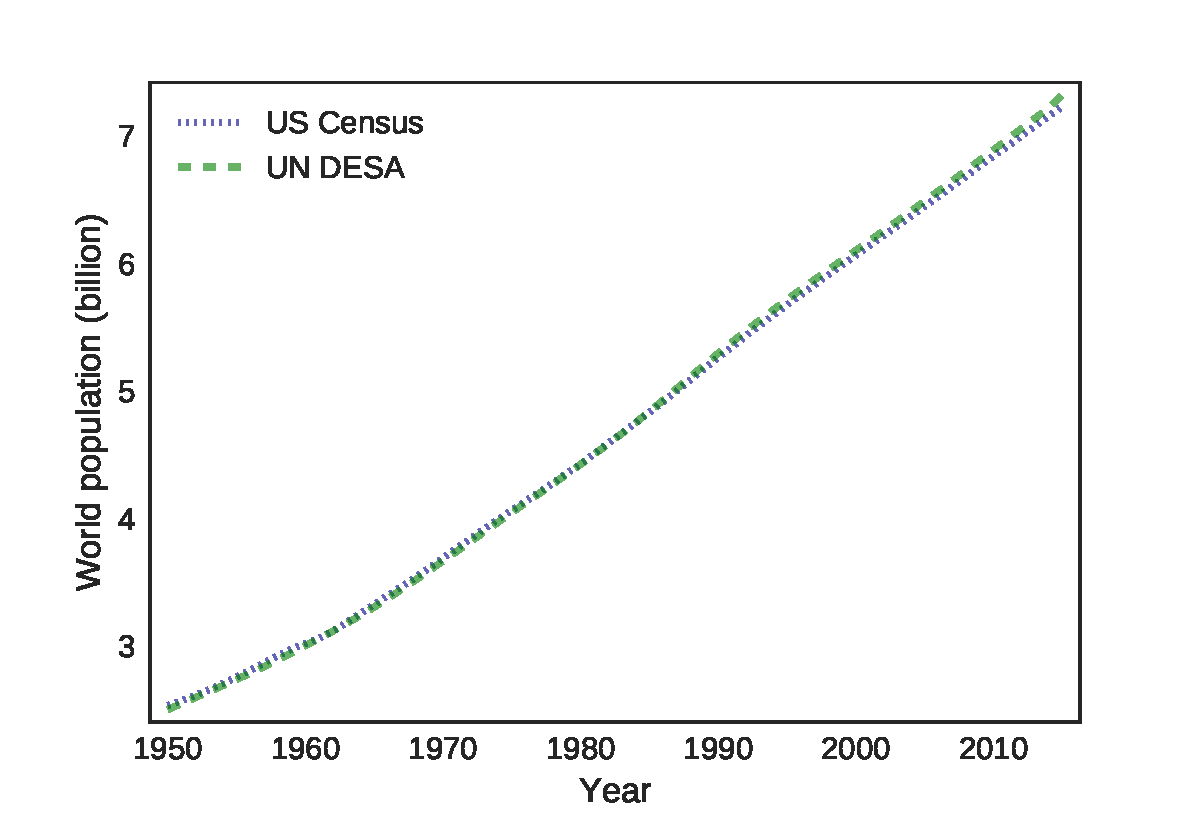
\includegraphics[height=3in]{figs/chap03-fig01.pdf}}
\caption{Estimates of world population, 1950--2015.}
\label{chap03-fig01}
\end{figure}

Figure~\ref{chap03-fig01} shows the result.  Generally the difference between the two estimates is less than 1\%.


\section{Constant growth model}

Suppose we want to predict world population growth over the next 50 or 100 years.  We can do that by developing a model that describes how population grows, fitting the model to the data we have so far, and then using the model to generate predictions.

In the next few sections I will demonstrate this process, starting with simple models, which will turn out not to sufficiently realistic to be credible, and gradually improving them.

Although there is some curvature in the plotted estimates, it looks like world population growth has been close to constant since 1960 or so.  As a starting place, we'll build a model with constant growth.

To fit the model to the data, we'll compute the average annual growth from 1950 to 2015.  Since the UN and Census data are so close, I'll use the Census data, again in terms of billions:

\begin{python}
census = table2.census / 1e9
\end{python}

We can select a value from a \py{Series} using bracket notation:

\begin{python}
census[1950]
\end{python}

So we can get the total growth during the interval like this:

\begin{python}
total_growth = census[2015] - census[1950]
\end{python}

But the values 2015 and 1950 are part of the data, so they should not be part of the program.  Putting values like these in the program is called {\bf hard coding}; it is considered bad practice because if the data changes in the future, we would have to modify the program.  For more about hard coding, see \url{https://en.wikipedia.org/wiki/Hard_coding}.

We can get the first and last year from the index, like this:

\begin{python}
first_year = census.index[0]
last_year = census.index[-1]
\end{python}

In brackets, \py{0} selects the first element from \py{census.index}, and \py{-1} selects the last element.  Now we can compute \py{total_growth} and \py{annual_growth}:

\begin{python}
total_growth = census[last_year] - census[first_year]
elapsed_time = last_year - first_year
annual_growth = total_growth / elapsed_time
\end{python}

The next step is to use this estimate to simulate population growth since 1950.

\section{Simulation}

First, we'll make a new \py{Series} object:

\begin{python}
model = Series([])
\end{python}

\py{Series} is a function that creates a new \py{Series} object.  The argument is a pair of empty brackets, \py{[]}, so initially the \py{Series} contains no values.

We can set the first value in the new \py{Series} by copying the first value from \py{census} (we'll get rid of the hard-coded dates soon):

\begin{python}
model[1950] = census[1950]
\end{python}

Then we can set the rest of the values by simulating annual growth:

\begin{python}
for year in arange(1951, 2016):
    model[year] = model[year-1] + annual_growth
\end{python}

The result from \py{arange} is an array of years from 1951 to 2015 (the second argument, 2016, is not included in the range).  In the model, the population each year is the number of the population during the previous year and \py{annual_growth}.

\begin{figure}
% chap03.ipynb.py
\centerline{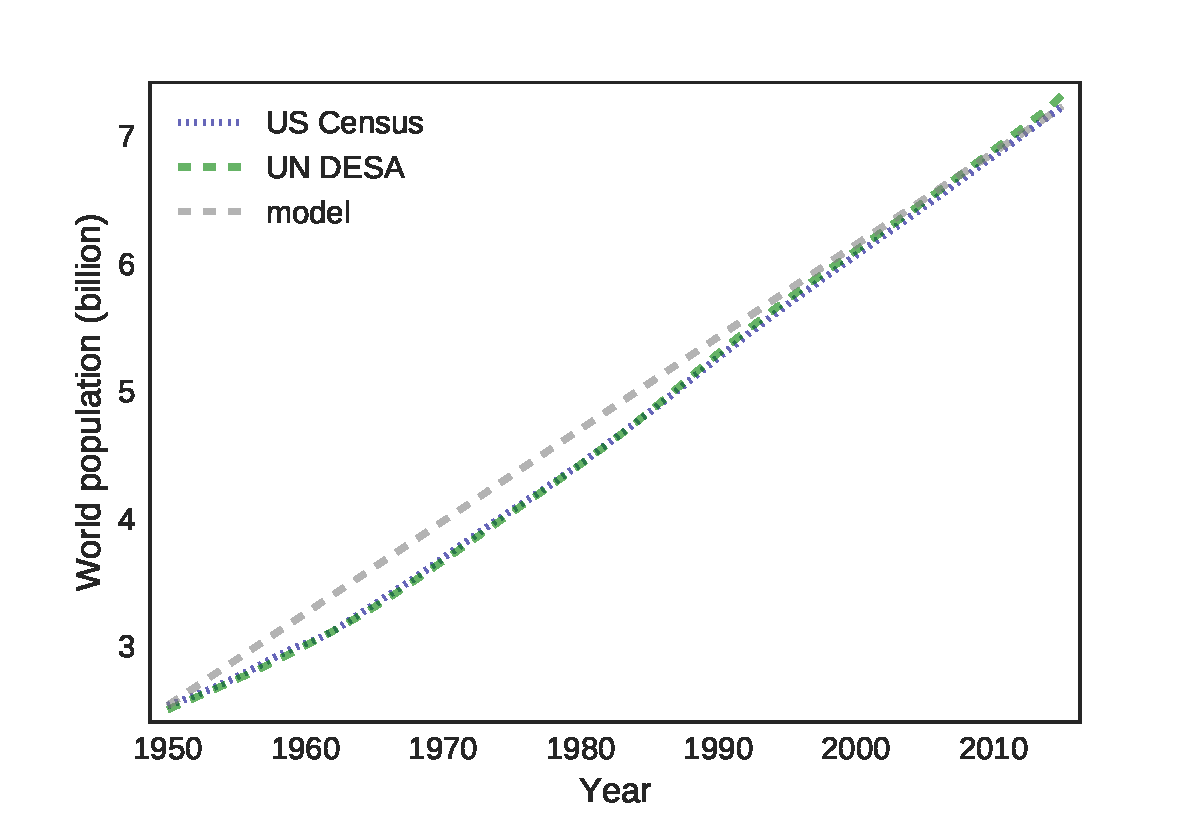
\includegraphics[height=3in]{figs/chap03-fig02.pdf}}
\caption{Estimates of world population, 1950--2015, and a constant growth model.}
\label{chap03-fig02}
\end{figure}

Figure~\ref{chap03-fig02} shows the result. The model does not fit the data particularly well from 1950 to the 1990, but after that, it's pretty good.  Nevertheless, there are problems:

\begin{itemize}

\item There is no plausible mechanism that could cause population growth to be constant from year to year.  Changes in population are determined the fraction of people who die and the fraction of people who give birth, so they should depend on the current population.

\item According to this model, we would expect the population to keep growing at the same rate forever, and that does not seem reasonable.

\end{itemize}

We'll try out some different models in the next few sections, but first let's clean up the code.


\section{Now with state objects}

First, let's put all the information we need to run the model into a state object:

\begin{python}
state = State(t0=first_year, t_end=last_year,
              init=census[first_year],
              annual_growth=annual_growth)
\end{python}

\py{t0} and \py{t_end} are the first and last years; \py{init} is the initial population, and \py{annual_growth} is the estimated annual growth.

Next we'll wrap the code from the previous section in a function:

\begin{python}
def run_model1(state):
    model = Series([])
    model[state.t0] = state.init
    for year in arange(state.t0+1, state.t_end+1):
        model[year] = model[year-1] + state.annual_growth
    state.model = model
\end{python}

When \py{run_model1} runs, it creates a new series that contains the result of the simulation, and stores it as a new state variable, \py{model}. 

To plot the results, we define a new function:

\begin{python}
def plot_model(state):
    newfig()
    plot_estimates()
    plot(state.model, '--', color='gray', label='model')
    decorate(xlabel='Year', 
             ylabel='World population (billion)',
             ylim=[0, 8])
\end{python}

There's nothing new there except \py{ylim}, which specifies the limits of the $y$ axis, in this case to make the figure look a little better.

Finally, we can run it like this.

\begin{python}
run_model1(state)
plot_model(state)
\end{python}

The results are the same as Figure~\ref{chap03-fig02}.

\section{Proportional model}

The biggest problem with the constant growth model is that it doesn't make any sense.    It is hard to imagine how people all over the world could conspire to keep the total constant from year to year.

On the order hand, if some fraction of the population dies each year, and some fraction gives birth, we can compute the net change in the population like this:

\begin{python}
def run_model2(state):
    model = Series([])
    model[state.t0] = state.init
    for year in arange(state.t0+1, state.t_end+1):
        births = state.birth_rate * model[year-1]
        deaths = state.death_rate * model[year-1]
        model[year] = model[year-1] + births - deaths
    state.model = model
\end{python}

Now we can choose the values of \py{birth_rate} and \py{death_rate} that best fit the data.  Without trying too hard, I chose:

\begin{python}
state.death_rate = 0.01
state.birth_rate = 0.027
\end{python}

Then I ran and plotted the model:

\begin{python}
run_model2(state)
plot_model(state)
\end{python}

\begin{figure}
% chap03.ipynb.py
\centerline{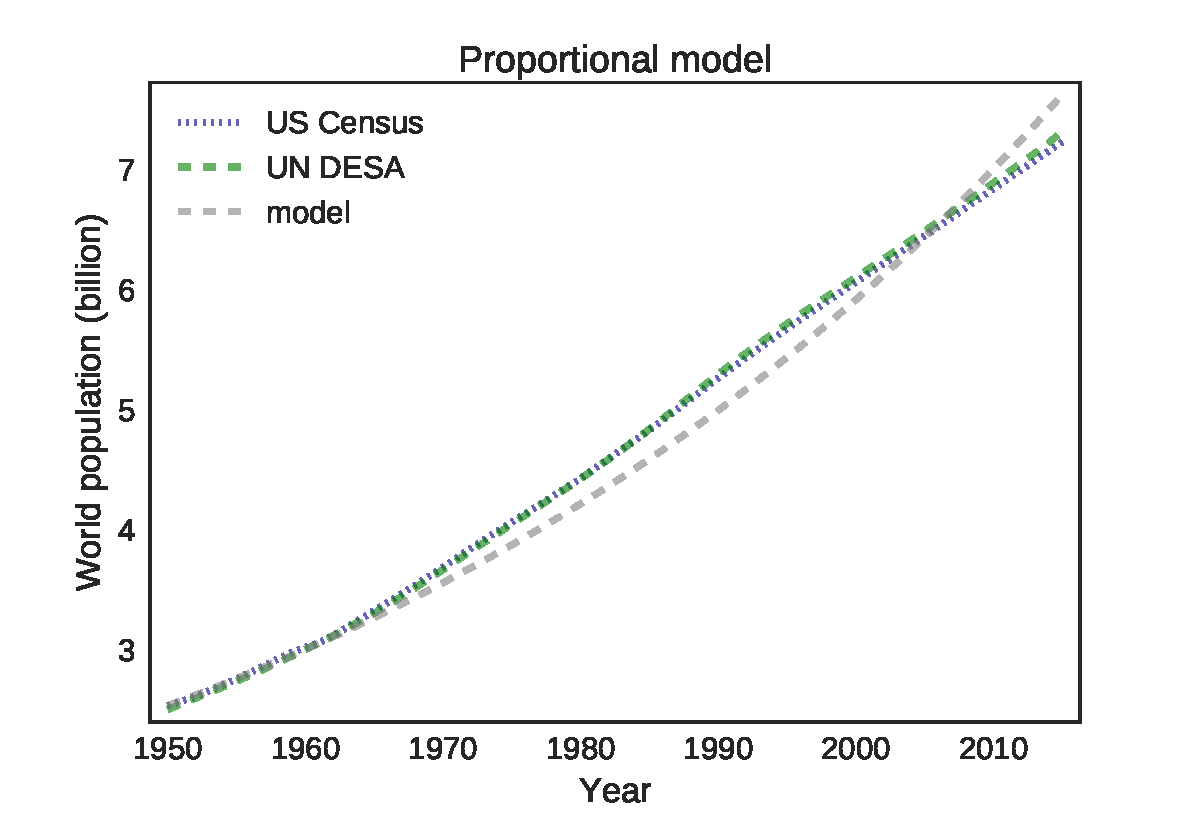
\includegraphics[height=3in]{figs/chap03-fig03.pdf}}
\caption{Estimates of world population, 1950--2015, and a proportional model.}
\label{chap03-fig03}
\end{figure}

Figure~\ref{chap03-fig03} shows the result.




\chapter{Explain}



\chapter{Design}

\backmatter
\printindex

\end{document}

\end{itemize}
